\chapter{Sound}
\label{p:wsl:s11}


\section{Introduction}
Now that we have studied the basics of longitudinal waves, we are ready to study sound waves in detail.

Have you ever thought about how amazing your sense of hearing is? It is actually pretty remarkable. There are many types of sounds: a car horn, a laughing baby, a barking dog, and somehow your brain can sort it all out. Though it seems complicated, it is rather simple to understand once you learn a very simple fact. Sound is a wave. So you can use everything you know about waves to explain sound.

\section{Characteristics of a Sound Wave}
%\begin{syllabus}
%\item The learner must be able to relate the pitch of a sound to the frequency of a sound %wave
%\item The learner must be able to relate the loudness of a sound to both the amplitude of a %sound wave and the sensitivity of the human ear
%\item The learner must be able to relate the quality of a sound to the harmonics that are %superposed in a given sound wave
%\item Notes: The human ear is more sensitive to some frequencies than to others. Loudness %thus depends on both the amplitude of a sound wave and its frequency (whether it lies in a %region where the ear is more or less sensitive).Make a link between the quality of the sound %and the standing waves produced in different musical instruments. The quality of the sound %produced by a particular instrument depends on which harmonics are superposed and in which %proportions.
%\end{syllabus}

Since sound is a wave, we can relate the properties of sound to the properties of a wave. The basic properties of sound are: pitch, loudness and tone.

\begin{figure}[h!tbp]
\begin{center}
%\scalebox{0.8}
%{
\begin{pspicture}(-5,-1)(5,1)%\psgrid
\psplot[xunit=0.0055,]{-360}{360}{x sin }
\psline[linestyle=dashed](-2,0)(2.5,0)
\psline[linestyle=dashed](-2,1)(2.5,1)
\psline[linestyle=dashed](-2,-1)(2.5,-1)
\psline{<->}(-2,-1.2)(-2,1.2)
\rput(-3.5,0){Sound A}
\end{pspicture}
%}
\end{center}

\begin{center}
%\scalebox{0.8}
%{
\begin{pspicture}(-5,-1)(5,2)%\psgrid
\psplot[xunit=0.0055,]{-360}{360}{-1 0.5 x mul sin mul}
\psline[linestyle=dashed](-2,0)(2.5,0)
\psline[linestyle=dashed](-2,1)(2.5,1)
\psline[linestyle=dashed](-2,-1)(2.5,-1)
\psline{<->}(-2,-1.2)(-2,1.2)
\rput(-3.5,0){Sound B}
\end{pspicture}
%}
\end{center}

\begin{center}
%\begin{minipage}{0.3\textwidth}
%\scalebox{0.8}
%{
\begin{pspicture}(-5,-1)(5,2)%\psgrid
\psplot[xunit=0.0055,]{-360}{360}{-1.5 0.5 x mul sin mul}
\psline[linestyle=dashed](-2,0)(2.5,0)
\psline[linestyle=dashed](-2,1)(2.5,1)
\psline[linestyle=dashed](-2,-1)(2.5,-1)
\psline{<->}(-2,-1.2)(-2,1.2)
\rput(-3.5,0){Sound C}
\end{pspicture}
%}
%\end{minipage}
\end{center}
\caption{Pitch and loudness of sound. Sound B has a \emph{lower} pitch (lower frequency) than Sound A and is \emph{softer} (smaller amplitude) than Sound C.}\label{fig:pitchetc}
\end{figure}

\subsection{Pitch}
The frequency of a sound wave is what your ear understands as pitch. A higher frequency sound has a higher pitch, and a lower frequency sound has a lower pitch. In Figure~\ref{fig:pitchetc} sound A has a higher pitch than sound B. For instance, the chirp of a bird would have a high pitch, but the roar of a lion would have a low pitch.

The human ear can detect a wide range of frequencies. Frequencies from 20 to 20 000 Hz are audible to the human ear. Any sound with a frequency below 20 Hz is known as an \textbf{infrasound} and any sound with a frequency above 20 000 Hz is known as an \textbf{ultrasound}.

Table~\ref{p:wsl:s11:rangeoff} lists the ranges of some common animals compared to humans.

\begin{table}[htbp]
\begin{center}
\caption{Range of frequencies }
\label{p:wsl:s11:rangeoff}
\begin{tabular}{|l|c|c|}\hline
&lower frequency (Hz) & upper frequency (Hz)\\\hline\hline
Humans & 20 & 20 000\\\hline
Dogs & 50 & 45 000\\\hline
Cats & 45 & 85 000\\\hline
Bats & 20 & 120 000\\\hline
Dolphins & 0,25 & 200 000\\\hline
Elephants & 5 & 10 000\\\hline
\hline
\end{tabular}
\end{center}
\end{table}

\Activity{Investigation}{Range of Wavelengths}{Using the information given in Table~\ref{p:wsl:s11:rangeoff}, calculate the lower and upper wavelengths that each species can hear. Assume the speed of sound in air is 344~\ms.}

\subsection{Loudness}
The amplitude of a sound wave determines its loudness or volume. A larger amplitude means a louder sound, and a smaller amplitude means a softer sound. In Figure~\ref{fig:pitchetc} sound C is louder than sound B. The vibration of a source sets the amplitude of a wave. It transmits energy into the medium through its vibration. More energetic vibration corresponds to larger amplitude. The molecules move back and forth more vigorously.

The loudness of a sound is also determined by the sensitivity of the ear. The human ear is more sensitive to some frequencies than to others. The volume we receive thus depends on both the amplitude of a sound wave and whether its frequency lies in a region where the ear is more or less sensitive.

\subsection{Tone}
Tone is a measure of the quality of the sound wave. For example, the quality of the sound produced in a particular musical instruments depends on which
harmonics are superposed and in which proportions. The harmonics are determined by the standing waves that are produced in the instrument. Chapter~\ref{p:wsl:pm11} will explain the physics of music in greater detail.

The quality (timbre) of the sound heard depends on the pattern of the incoming vibrations, i.e. the \textit{shape} of the sound wave. The more irregular the vibrations, the more jagged is the shape of the sound wave and the harsher is the sound heard.

\section{Speed of Sound}
The speed of sound depends on the medium the sound is travelling in. Sound travels faster in solids than in liquids, and faster in liquids than in gases. This is because the density of solids is higher than that of liquids which means that the particles are closer together. Sound can be transmitted more easily.

The speed of sound also depends on the temperature of the medium. The hotter the medium is, the faster its particles move and therefore the quicker the sound will travel through the medium. When we heat a substance, the particles in that substance have more kinetic energy and vibrate or move faster. Sound can therefore be transmitted more easily and quickly in hotter substances.

Sound waves are pressure waves. The speed of sound will therefore be influenced by the pressure of the medium through which it is travelling. At sea level the air pressure is higher than high up on a mountain. Sound will travel faster at sea level where the air pressure is higher than it would at places high above sea level.

\Definition{Speed of sound}{The speed of sound in air, at sea level, at a temperature of 21\deg C and under normal atmospheric conditions, is 344~\ms.}

\Exercise{Sound frequency and amplitude}{
\begin{minipage}{0.49\textwidth}
Study the following diagram representing a musical note.
Redraw the diagram for a note
\begin{enumerate}
\item with a higher pitch
\item that is louder
\item that is softer
\end{enumerate}
\end{minipage}
\begin{minipage}{0.49\textwidth}
\begin{pspicture}(-3,-1)(5,1)%\psgrid
\psplot[xunit=0.0055,]{-360}{360}{x sin }
\psline[linestyle=dashed](-2,0)(2.5,0)
\psline[linestyle=dashed](-2,1)(2.5,1)
\psline[linestyle=dashed](-2,-1)(2.5,-1)
\psline{<->}(-2,-1.2)(-2,1.2)
\end{pspicture}
\end{minipage}
\practiceinfo

\begin{tabular}[h]{cccccc}
(1.) 00sj & (2.) 00sk & (3.) 00sm & 
 \end{tabular}
}
Veritasium video on sound: SIYAVULA-VIDEO:http://cnx.org/content/m39034/latest/#sound-1
\section{Physics of the Ear and Hearing}
%\begin{syllabus}
%\item The learner must be able to identify the important features on simple diagram of the human ear showing the outer ear, eardrum, ear canal, ossicles, inner ear and auditory nerve.
%\item The learner must be able to refer to the features listed above to explain how sound is transmitted from the outer ear to the auditory nerve, from where a signal is sent to the brain.
%\item The learner must be able to state that the intensity of sound is measured in decibels (dB).
%\item The learner must be able to indicate the relative intensities of a variety of sounds
%\item The learner must be able to explain the dangers of exposure to very loud sounds and what can be done to reduce these dangers.
%\item Notes: Learners should get a table of intensities for a variety of different sounds. They should know that permanent damage can be caused by exposure to very loud sounds. This is an opportunity to discuss the importance of safety equipment such as ear protectors for workers in loud environments, e.g. those who use jack hammers or direct airplanes to their parking bays.
%\end{syllabus}

\begin{center}
\begin{figure}[H]
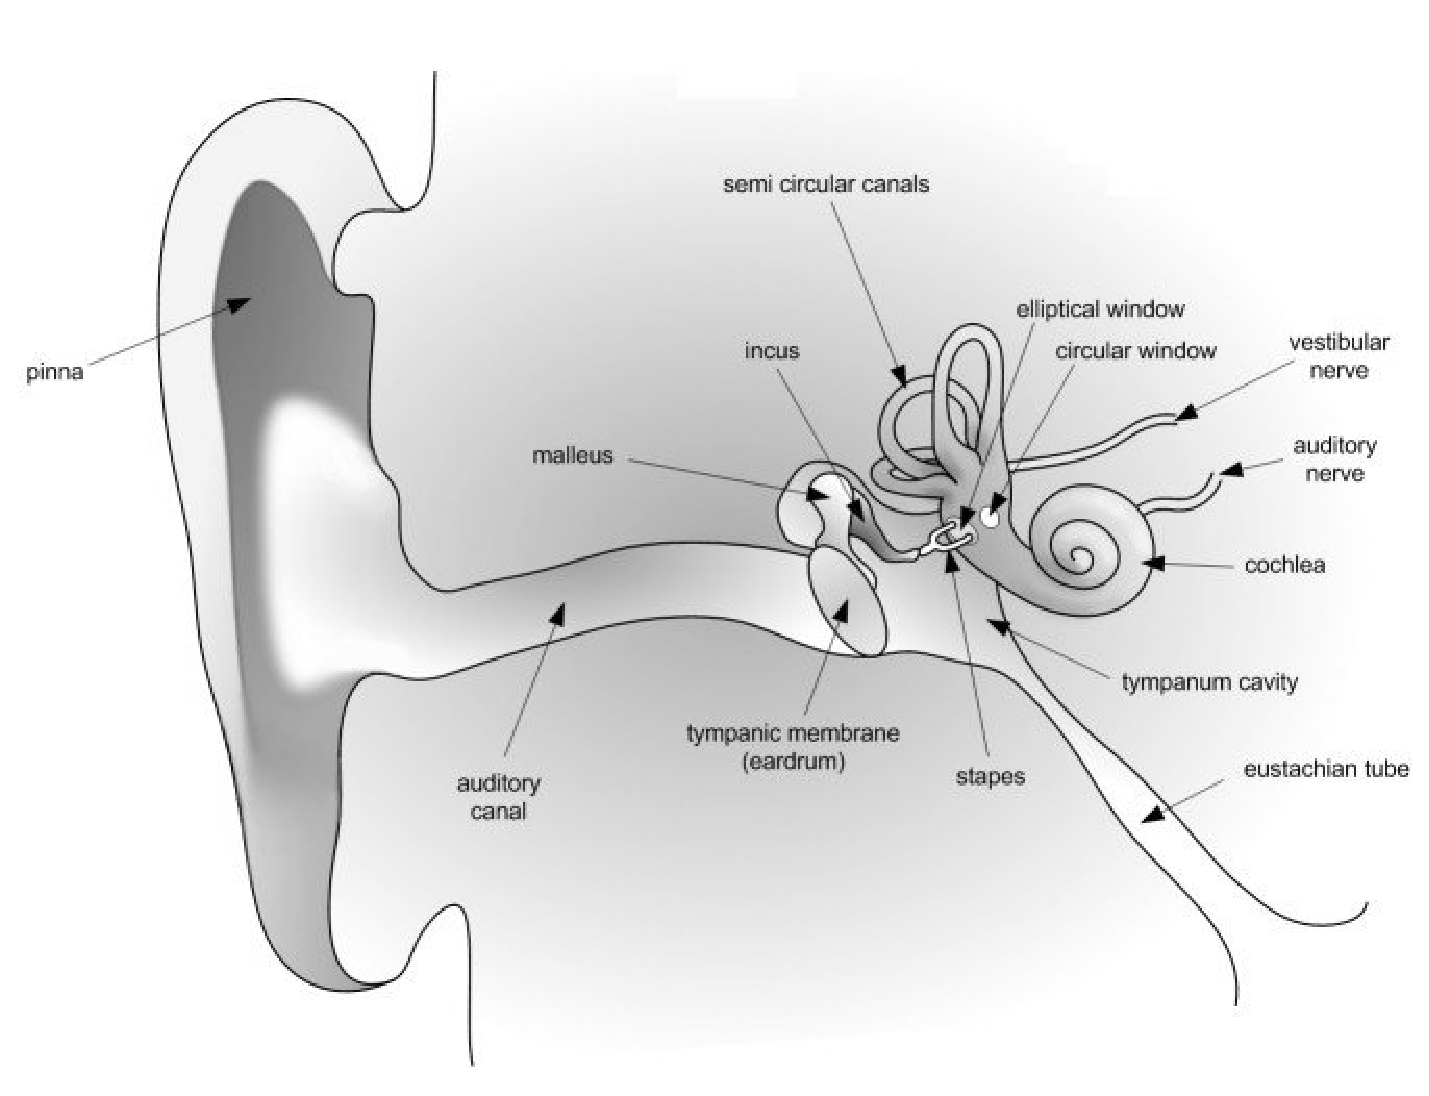
\includegraphics[width=0.65\textwidth]{../HumanEar-GrayScale.eps}
\caption{Diagram of the human ear. }
\label{Human Ear}
\end{figure}
\end{center}

The human ear is divided into three main sections: the outer, middle,
and inner ear. Let's follow the journey of a sound wave from the pinna (outermost part) to the auditory nerve (innermost part) which transmits a signal to the brain. The pinna  is the part of the ear we typically think of when we refer to the ear. Its main
function is to collect and focus an incident sound wave. The wave
then travels through the ear canal until it meets the eardrum. The
pressure fluctuations of the sound wave make the eardrum vibrate.
The three very small bones of the middle ear, the malleus (hammer),
the incus (anvil), and the stapes (stirrup), transmit the signal through
to the elliptical window. The elliptical window is the beginning of the
inner ear. From the elliptical window the sound waves are transmitted through the liquid
in the inner ear and interpreted as sounds by the brain.
The inner ear, made of the semicircular canals, the cochlea,
and the auditory nerve, is filled with fluid. The fluid allows the body to
detect quick movements and maintain balance. The snail-shaped cochlea
is covered in nerve cells. There are more than 25 000 hairlike
nerve cells. Different nerve cells vibrate with different
frequencies. When a nerve cell vibrates, it releases electrical impulses
to the auditory nerve. The impulses are sent to the brain through the
auditory nerve and understood as sound.

\subsection{Intensity of Sound}
Intensity is one indicator of amplitude. Intensity is the energy transmitted over a unit of area each second.

\Extension{Intensity}{Intensity is defined as:
\nequ{\rm{Intensity}=\frac{\rm{energy}}{\rm{time} \times \rm{area}}=\frac{\rm{power}}{\rm{area}}}

By the definition of intensity, we can see that the units of intensity are
\nequ{\frac{\rm{Joules}}{\mathrm{s \cdot m^{2}}}=\frac{\rm{Watts}}{\rm{m}^{2}}}
}

The unit of intensity is the \textbf{decibel} (symbol: dB). This reduces to an SI equivalent of $\mathrm{W \cdot m^{-2}}$.

The average threshold of hearing is $10^{-12}~\mathrm{W\cdot m^{-2}}$. Below this intensity, the sound is too soft for the ear to hear. The threshold of pain is $1.0~\mathrm{W\cdot m^{-2}}$. Above this intensity a sound is so loud it becomes uncomfortable for
the ear.

Notice that there is a factor of $10^{12}$ between the thresholds of
hearing and pain. This is one reason we define the decibel (dB) scale.

\Extension{dB Scale}{The intensity in dB of a sound of intensity $I$, is given by:
\begin{equation}
\beta =10~\log\frac{I}{I_o} \qquad \qquad {I_o}=10^{-12}~\mathrm{W\cdot m^{-2}}
\end{equation}}

In this way we can compress the whole hearing intensity scale into a
range from 0 dB to 120 dB.

\begin{table}[H]
\begin{center}
\caption{Examples of sound intensities.}
\label{p:wsl:s11:intensity}
\begin{tabular}{|l|c|c|}\hline
\textbf{Source}&\textbf{Intensity} (dB) & \textbf{Times greater than hearing threshold}\\\hline
& & \\
Rocket Launch &180 & $10^{18}$\\
Jet Plane & 140 & $10^{14}$ \\
Threshold of Pain & 120 & $10^{12}$\\
Rock Band & 110 & $10^{11}$\\
Subway Train & 90 & $10^{9}$\\
Factory & 80 & $10^{8}$\\
City Traffic & 70 & $10^{7}$\\
Normal Conversation & 60 & $10^{6}$\\
Library & 40 & $10^{4}$\\
Whisper & 20 & $10^{2}$\\
Threshold of hearing & 0 & 0\\
\hline
\end{tabular}
\end{center}
\end{table}

Notice that there are sounds which exceed the threshold
of pain. Exposure to these sounds can cause immediate damage to hearing.
In fact, exposure to sounds from
80 dB and above can damage hearing over time. Measures
can be taken to avoid damage, such as wearing earplugs
or ear muffs. Limiting exposure time and
increasing distance between you and the source are also
important steps for protecting your hearing.

\Activity{Discussion}{Importance of Safety Equipment}{Working in groups of 5, discuss the importance of safety equipment such as ear protectors for workers in loud environments, e.g. those who use jack hammers or direct aeroplanes to their parking bays. Write up your conclusions in a one page report. Some prior research into the importance of safety equipment might be necessary to complete this group discussion.}
Phet simulation on sound: SIYAVULA-SIMULATION:http://cnx.org/content/m39035/latest/#id63458
\section{Ultrasound}
%\begin{syllabus}
%\item The learner must be able to describe sound with frequencies higher than 20 kHz as ultrasound, up to about 100 kHz.
%\item The learner must be able to explain how an image can be created using ultrasound based on the fact that when a wave encounters a boundary between two media, part of the wave is reflected and part is transmitted.
%\item The learner must be able to describe some of the medical benefits and uses of ultrasound, e.g. safety, diagnosis, treatment, pregnancy.
%\item Notes: Make a link to Grade 10, reflection and transmission at a boundary. When an ultrasound wave travels inside an object comprising different materials such as the human body, each time it encounters a boundary, e.g. between bone and muscle, or muscle and fat, part of the wave is reflected and part of it is transmitted. The reflected rays are detected and used to construct an image of the object.
%\end{syllabus}

Ultrasound is sound with a frequency that is higher than 20 kHz. Some animals, such as dogs, dolphins, and bats, have an upper limit that is greater than that of the human ear and can hear ultrasound.

The most common use of ultrasound is to create images, and has industrial and medical applications. The use of ultrasound to create images is based on the reflection and transmission of a wave at a boundary. When an ultrasound wave travels inside an object that is made up of different materials such as the human body, each time it encounters a boundary, e.g. between bone and muscle, or muscle and fat, part of the wave is reflected and part of it is transmitted. The reflected rays are detected and used to construct an image of the object.

Ultrasound in medicine can visualise muscle and soft tissue, making them useful for scanning the organs, and is commonly used during pregnancy. Ultrasound is a safe, non-invasive method of looking inside the human body.

Ultrasound sources may be used to generate local heating in biological tissue, with applications in physical therapy and cancer treatment. Focussed ultrasound sources may be used to break up kidney stones.

Ultrasonic cleaners, sometimes called supersonic cleaners, are used at frequencies from 20-40 kHz for jewellery, lenses and other optical parts, watches, dental instruments, surgical instruments and industrial parts.
These cleaners consist of containers with a fluid in which the object to be cleaned is placed. Ultrasonic waves are then sent into the fluid. The main mechanism for cleaning action in an ultrasonic cleaner is actually the energy released from the collapse of millions of microscopic bubbles occurring in the liquid of the cleaner.

\begin{IFact}{Ultrasound generator/speaker systems are sold with claims that they frighten away rodents and insects, but there is no scientific evidence that the devices work; controlled tests have shown that rodents quickly learn that the speakers are harmless.
}\end{IFact}

%\begin{IFact}
%{Medical ultrasonography was invented in 1953 at Lund University in Sweden by cardiologist Inge Edler and Carl Hellmuth %Hertz, the son of Gustav Ludwig Hertz, who was a graduate student at the department for nuclear physics.}
%\end{IFact}

%\begin{IFact}{In echo-sounding the reflections from ultrasound pulses that are bounced off objects (for example the bottom of the sea, fish etc.) are picked up. The reflections are timed and since their speed is known, the distance to the object can be found. This information can be built into a picture of the object that reflects the ultrasound pulses.}
%\end{IFact}

%In medical scanning, the ultrasound is reflected off each tissue boundary and is picked up. %The reflections are used to build up a picture showing what is inside the body, for example %in pre-natal scans. Some of the ultrasound energy is absorbed by the body, but it is much %less damaging than x-rays.

\section{SONAR}

\begin{center}
\scalebox{0.8} % Change this value to rescale the drawing.
{
\begin{pspicture}(0,-3.93)(11.42,3.91)
\definecolor{color78b}{rgb}{0.6,0.6,0.6}
\psbezier[linewidth=0.04](0.52,-1.6283582)(3.3282945,-0.05)(4.980751,-1.0964925)(5.8,-2.11)(6.619249,-3.1235075)(8.99,-3.91)(10.64,-3.71)
\psbezier[linewidth=0.04,fillstyle=solid,fillcolor=color78b](1.94,2.61)(1.9801459,1.77)(1.84,1.17)(2.44,1.15)(3.04,1.13)(6.68,1.01)(7.358321,1.29)(8.036642,1.57)(9.52,2.81)(8.58,2.59)(7.64,2.37)(1.96,2.43)(1.92,2.59)
\psline[linewidth=0.04cm](2.52,2.49)(2.52,3.27)
\psline[linewidth=0.04cm](2.52,3.27)(4.44,3.27)
\psline[linewidth=0.04cm](4.44,3.27)(4.44,2.45)
\psline[linewidth=0.04cm](3.14,3.81)(3.14,3.27)
\psline[linewidth=0.04cm](3.76,3.81)(3.76,3.27)
\psellipse[linewidth=0.04,dimen=outer](3.45,3.82)(0.33,0.09)
\pscircle[linewidth=0.04,dimen=outer,fillstyle=solid,fillcolor=color78b](2.74,3.05){0.14}
\pscircle[linewidth=0.04,dimen=outer,fillstyle=solid,fillcolor=color78b](3.18,3.05){0.14}
\pscircle[linewidth=0.04,dimen=outer,fillstyle=solid,fillcolor=color78b](3.7,3.05){0.14}
\pscircle[linewidth=0.04,dimen=outer,fillstyle=solid,fillcolor=color78b](4.12,3.05){0.14}
\pscircle[linewidth=0.04,dimen=outer,fillstyle=solid,fillcolor=color78b](2.96,2.77){0.14}
\pscircle[linewidth=0.04,dimen=outer,fillstyle=solid,fillcolor=color78b](3.44,2.77){0.14}
\pscircle[linewidth=0.04,dimen=outer,fillstyle=solid,fillcolor=color78b](3.9,2.75){0.14}
\rput(7.5798435,2.24){SAS Sonar}
\psframe[linewidth=0.04,dimen=outer,fillstyle=solid](3.24,1.15)(3.02,1.05)
\psframe[linewidth=0.04,dimen=outer,fillstyle=solid](4.58,1.13)(4.36,1.03)
\pscustom[linewidth=0.04]
{
\newpath
\moveto(9.94,1.31)
}
\psline[linewidth=0.04cm](0.0,1.61)(11.4,1.61)
\psline[linewidth=0.04cm](3.12,1.15)(3.76,-0.85)
\psline[linewidth=0.04cm](3.76,-0.85)(4.48,1.13)
\psline[linewidth=0.04cm](3.2972062,0.25496995)(3.4476187,0.11434252)
\psline[linewidth=0.04cm](3.4476187,0.11434252)(3.4875562,0.316345)
\psline[linewidth=0.04cm](4.229458,0.10226333)(4.187863,0.30393106)
\psline[linewidth=0.04cm](4.187863,0.30393106)(4.0386105,0.1620733)
\rput(3.2217188,-1.2){seabed}
\rput(1.949375,0.62){transmitter}
\rput(5.47,0.62){receiver}
\psline[linewidth=0.04cm,arrowsize=0.05291667cm 2.0,arrowlength=1.4,arrowinset=0.4]{->}(2.56,0.81)(3.0,1.03)
\psline[linewidth=0.04cm,arrowsize=0.05291667cm 2.0,arrowlength=1.4,arrowinset=0.4]{->}(4.92,0.79)(4.64,1.03)
%\psline[linewidth=0.04cm,arrowsize=0.05291667cm %2.0,arrowlength=1.4,arrowinset=0.4]{->}(6.36,-0.09)(6.36,-0.09)
\rput(7.020781,-0.46){sea}
\end{pspicture}
}
\end{center}

Ships on the ocean make use of the reflecting properties of sound waves to determine the depth of the ocean. A sound wave is transmitted and bounces off the seabed. Because the speed of sound is known and the time lapse between sending and receiving the sound can be measured, the distance from the ship to the bottom of the ocean can be determined, This is called sonar, which stands from \textbf{So}und \textbf{N}avigation \textbf{A}nd \textbf{R}anging.

\subsection{Echolocation}
Animals like dolphins and bats make use of sounds waves to find their way. Just like ships on the ocean, bats use sonar to navigate. Ultrasound waves that are sent out are reflected off the objects around the animal. Bats, or dolphins, then use the reflected sounds to form a ``picture'' of their surroundings. This is called echolocation.

\begin{wex}{SONAR}
{A ship sends a signal to the bottom of the ocean to determine the depth of the ocean. The speed of sound in sea water is 1450 $\rm{m.s^{-1}}$ If the signal is received 1,5 seconds later, how deep is the ocean at that point?}
{
\westep{Identify what is given and what is being asked:}
\begin{eqnarray*}
s &=& 1450 \ \rm{m.s^{-1}}\\
t &=& 1,5 \ \rm{s} \ \rm{there \ and \ back}\\
\therefore t &= & 0,75 \ \rm{s} \ \rm{one \ way}\\
d &=& ?
\end{eqnarray*}

\westep{Calculate the distance:}
\begin{eqnarray*}
\rm{Distance} &=& \rm{speed} \times \rm{time} \\
d &=& s \times t \\
&=& 1450 m.s^{-1} \times 0,75 s \\
&=& 1087,5 \ \rm{m}
\end{eqnarray*}

}
\end{wex}

Presentation on sound: SIYAVULA-PRESENTATION:http://cnx.org/content/m39035/latest/#slidesharefigure

\summary{aaa}
\begin{enumerate}
\item Sound waves are longitudinal waves
\item The \textbf{frequency} of a sound is an indication of how high or low the \emph{pitch} of the sound is.
\item The human ear can hear frequencies from 20 to 20~000 Hz. \\
\textbf{Infrasound} waves have frequencies lower than 20 Hz. \\
\textbf{Ultrasound} waves have frequencies higher than 20~000 Hz.
\item The \textbf{amplitude} of a sound determines its \emph{loudness} or volume.
\item The \textbf{tone} is a measure of the \emph{quality} of a sound wave.
\item The speed of sound in air is around 340 m.s$^{-1}$. It is dependent on the temperature, height above sea level and the phase of the medium through which it is travelling.
\item Sound travels faster when the medium is hot.
\item Sound travels faster in a solid than a liquid and faster in a liquid than in a gas.
\item Sound travels faster at sea level where the air pressure is higher.
\item The intensity of a sound is the energy transmitted over a certain area. Intensity is a measure of frequency.
\item Ultrasound can be used to form pictures of things we cannot see, like unborn babies or tumors.
\item Echolocation is used by animals such as dolphins and bats to ``see'' their surroundings by using ultrasound.
\item Ships use sonar to determine how deep the ocean is or to locate shoals of fish.
\end{enumerate}

\begin{eocexercises}{}
\renewcommand{\labelenumii}{\Alph{enumii}}
\begin{enumerate}

\item Choose a word from column B that best describes the concept in column A. \\
\begin{center}
\begin{tabular}{ll}
\textbf{Column A} & \textbf{Column B} \\ \hline
pitch of sound \ \ \ & amplitude \\
loudness of sound \ \ \ \ \ \ \ \ \ & frequency \\
quality of sound \ \ \ & speed \\
& waveform \\
\end{tabular}
\end{center}

\item A tuning fork, a violin string and a loudspeaker are producing sounds. This is because they are all in a state of:
\begin{enumerate}
\item compression
\item rarefaction
\item rotation
\item tension
\item vibration
\end{enumerate}

\item What would a drummer do to make the sound of a drum give a note of lower pitch?
\begin{enumerate}
\item hit the drum harder
\item hit the drum less hard
\item hit the drum near the edge
\item loosen the drum skin
\item tighten the drum skin
\end{enumerate}

\item What is the approximate range of audible frequencies for a healthy human?
\begin{enumerate}
\item 0.2 Hz $\rightarrow$ 200 Hz
\item 2 Hz $\rightarrow$ 2 000 Hz
\item 20 Hz $\rightarrow$ 20 000 Hz
\item 200 Hz $\rightarrow$ 200 000 Hz
\item 2 000 Hz $\rightarrow$ 2 000 000 Hz
\end{enumerate}

\item X and Y are different wave motions. In air, X travels much faster than Y but has a much shorter wavelength. Which types of wave motion could X and Y be?

\begin{tabular}{lll}
& \underline{X} & \underline{Y}\\
A & microwaves & red light\\
B & radio & infra red\\
C & red light & sound\\
D & sound & ultraviolet\\
E & ultraviolet & radio\\
\end{tabular}

\item Astronauts are in a spaceship orbiting the moon. They see an explosion on the surface of the moon. Why can they not hear the explosion?
\begin{enumerate}
\item explosions do not occur in space
\item sound cannot travel through a vacuum
\item sound is reflected away from the spaceship
\item sound travels too quickly in space to affect the ear drum
\item the spaceship would be moving at a supersonic speed
\end{enumerate}

\item A man stands between two cliffs as shown in the diagram and claps his hands once.

% Generated with LaTeXDraw 1.9.3
% Tue Oct 23 18:53:18 SAST 2007
% \usepackage[usenames,dvipsnames]{pstricks}
% \usepackage{epsfig}
% \usepackage{pst-grad} % For gradients
% \usepackage{pst-plot} % For axes
%\scalebox{1} % Change this value to rescale the drawing.
\begin{center}
{
\begin{pspicture}(0,-1.0985937)(7.6665626,1.1185937)
\psline[linewidth=0.04cm](1.260625,0.92140627)(1.260625,-1.0785937)
\psline[linewidth=0.04cm](6.260625,0.94140625)(6.260625,-1.0585938)
%\usefont{T1}{ptm}{m}{n}
\rput(0.4575,0.47140625){cliff 1}
%\usefont{T1}{ptm}{m}{n}
\rput(7.1339064,0.49140626){cliff 2}
\psline[linewidth=0.04cm](1.260625,-1.0785937)(6.240625,-1.0585938)
\psline[linewidth=0.04cm](4.260625,0.88140625)(4.240625,0.52140623)
\psline[linewidth=0.04cm,arrowsize=0.1029cm 2.04,arrowlength=1.44,arrowinset=0.4]{<->}(1.240625,0.70140624)(4.240625,0.70140624)
\psline[linewidth=0.04cm,arrowsize=0.0929cm 2.05,arrowlength=1.45,arrowinset=0.4]{<->}(4.300625,0.70140624)(6.260625,0.70140624)
\pscircle[linewidth=0.04,dimen=outer](4.250625,0.21140625){0.25}
\psline[linewidth=0.04cm](4.240625,-0.05859375)(4.240625,-0.6585938)
\psline[linewidth=0.04cm](4.240625,-0.6585938)(3.940625,-1.0585938)
\psline[linewidth=0.04cm](4.240625,-0.6585938)(4.540625,-1.0585938)
\psline[linewidth=0.04cm](4.040625,-0.25859374)(4.440625,-0.25859374)
%\usefont{T1}{ptm}{m}{n}
\rput(2.6015625,0.94140625){\footnotesize 165 m}
%\usefont{T1}{ptm}{m}{n}
\rput(5.2015624,0.94140625){\footnotesize 110 m}
\end{pspicture}
}
\end{center}

Assuming that the velocity of sound is 330 m.s$^{-1}$, what will be the time interval between the two loudest echoes?
\begin{enumerate}
\item $\frac{1}{6}$ s
\item $\frac{5}{6}$ s
\item $\frac{1}{3}$ s
\item $1$ s
\item $\frac{2}{3}$ s
\end{enumerate}

\item A dolphin emits an ultrasonic wave with frequency of 0,15 MHz. The speed of the ultrasonic wave in water is 1 500 m.s$^{-1}$. What is the wavelength of this wave in water?
\begin{enumerate}
\item 0.1 mm
\item 1 cm
\item 10 cm
\item 10 m
\item 100 m
\end{enumerate}

\comment{
\item A stamp collecter is using a magnifying glass to see a stamp more clearly.
Where should the stamp be placed?

% Generated with LaTeXDraw 1.9.3
% Tue Oct 23 20:07:16 SAST 2007
% \usepackage[usenames,dvipsnames]{pstricks}
% \usepackage{epsfig}
% \usepackage{pst-grad} % For gradients
% \usepackage{pst-plot} % For axes
%\scalebox{1} % Change this value to rescale the drawing.
\begin{center}
{
\begin{pspicture}(0,-2.3428125)(11.05875,2.3228126)
\definecolor{color1683b}{rgb}{0.011764705882352941,0.027450980392156862,0.027450980392156862}
\definecolor{color2300b}{rgb}{0.03529411764705882,0.01568627450980392,0.01568627450980392}
\pspolygon[linewidth=0.04](1.26,-1.0971875)(1.26,0.44535795)(2.32,0.5828125)(2.32,-0.95973295)(2.32,-0.95973295)(2.32,-0.95973295)(2.32,-0.95973295)
\pscustom[linewidth=0.04]
{
\newpath
\moveto(4.04,2.3028126)
}
\pscustom[linewidth=0.04]
{
\newpath
\moveto(1.26,0.6028125)
\lineto(1.3,0.5928125)
\curveto(1.32,0.5878125)(1.365,0.5878125)(1.39,0.5928125)
\curveto(1.415,0.5978125)(1.455,0.6228125)(1.47,0.6428125)
\curveto(1.485,0.6628125)(1.53,0.6728125)(1.56,0.6628125)
\curveto(1.59,0.6528125)(1.645,0.6328125)(1.67,0.6228125)
\curveto(1.695,0.6128125)(1.735,0.6128125)(1.75,0.6228125)
\curveto(1.765,0.6328125)(1.8,0.6378125)(1.82,0.6328125)
\curveto(1.84,0.6278125)(1.885,0.6178125)(1.91,0.6128125)
\curveto(1.935,0.6078125)(1.975,0.6228125)(1.99,0.6428125)
\curveto(2.005,0.6628125)(2.05,0.6728125)(2.08,0.6628125)
\curveto(2.11,0.6528125)(2.165,0.6478125)(2.19,0.6528125)
\curveto(2.215,0.6578125)(2.26,0.6778125)(2.28,0.6928125)
\curveto(2.3,0.7078125)(2.355,0.7128125)(2.39,0.7028125)
\curveto(2.425,0.6928125)(2.46,0.6678125)(2.46,0.6528125)
\curveto(2.46,0.6378125)(2.445,0.5978125)(2.43,0.5728125)
\curveto(2.415,0.5478125)(2.405,0.4928125)(2.41,0.4628125)
\curveto(2.415,0.4328125)(2.43,0.3828125)(2.44,0.3628125)
\curveto(2.45,0.3428125)(2.45,0.3128125)(2.44,0.3028125)
\curveto(2.43,0.2928125)(2.42,0.2628125)(2.42,0.2428125)
\curveto(2.42,0.2228125)(2.42,0.1878125)(2.42,0.1728125)
\curveto(2.42,0.1578125)(2.42,0.1178125)(2.42,0.0928125)
\curveto(2.42,0.0678125)(2.425,0.0278125)(2.43,0.0128125)
\curveto(2.435,-0.0021875)(2.445,-0.0421875)(2.45,-0.0671875)
\curveto(2.455,-0.0921875)(2.46,-0.1221875)(2.46,-0.1271875)
\curveto(2.46,-0.1321875)(2.455,-0.1671875)(2.45,-0.1971875)
\curveto(2.445,-0.2271875)(2.425,-0.2771875)(2.41,-0.2971875)
\curveto(2.395,-0.3171875)(2.39,-0.3571875)(2.4,-0.3771875)
\curveto(2.41,-0.3971875)(2.44,-0.4221875)(2.46,-0.4271875)
\curveto(2.48,-0.4321875)(2.47,-0.4571875)(2.44,-0.4771875)
\curveto(2.41,-0.4971875)(2.39,-0.5321875)(2.4,-0.5471875)
\curveto(2.41,-0.5621875)(2.42,-0.6071875)(2.42,-0.6371875)
\curveto(2.42,-0.6671875)(2.415,-0.7121875)(2.41,-0.7271875)
\curveto(2.405,-0.7421875)(2.415,-0.7721875)(2.43,-0.7871875)
\curveto(2.445,-0.8021875)(2.445,-0.8421875)(2.43,-0.8671875)
\curveto(2.415,-0.8921875)(2.4,-0.9421875)(2.4,-0.9671875)
\curveto(2.4,-0.9921875)(2.39,-1.0321875)(2.38,-1.0471874)
\curveto(2.37,-1.0621876)(2.34,-1.0871875)(2.32,-1.0971875)
\curveto(2.3,-1.1071875)(2.25,-1.1071875)(2.22,-1.0971875)
\curveto(2.19,-1.0871875)(2.14,-1.0771875)(2.12,-1.0771875)
\curveto(2.1,-1.0771875)(2.06,-1.0871875)(2.04,-1.0971875)
\curveto(2.02,-1.1071875)(1.97,-1.1221875)(1.94,-1.1271875)
\curveto(1.91,-1.1321875)(1.855,-1.1321875)(1.83,-1.1271875)
\curveto(1.805,-1.1221875)(1.75,-1.1271875)(1.72,-1.1371875)
\curveto(1.69,-1.1471875)(1.64,-1.1671875)(1.62,-1.1771874)
\curveto(1.6,-1.1871876)(1.555,-1.1971875)(1.53,-1.1971875)
\curveto(1.505,-1.1971875)(1.455,-1.1921875)(1.43,-1.1871876)
\curveto(1.405,-1.1821876)(1.35,-1.1771874)(1.32,-1.1771874)
\curveto(1.29,-1.1771874)(1.24,-1.1821876)(1.22,-1.1871876)
\curveto(1.2,-1.1921875)(1.17,-1.1771874)(1.16,-1.1571875)
\curveto(1.15,-1.1371875)(1.145,-1.0971875)(1.15,-1.0771875)
\curveto(1.155,-1.0571876)(1.15,-1.0171875)(1.14,-0.9971875)
\curveto(1.13,-0.9771875)(1.115,-0.9221875)(1.11,-0.8871875)
\curveto(1.105,-0.8521875)(1.115,-0.7921875)(1.13,-0.7671875)
\curveto(1.145,-0.7421875)(1.16,-0.7021875)(1.16,-0.6871875)
\curveto(1.16,-0.6721875)(1.145,-0.6271875)(1.13,-0.5971875)
\curveto(1.115,-0.5671875)(1.105,-0.5171875)(1.11,-0.4971875)
\curveto(1.115,-0.4771875)(1.125,-0.4371875)(1.13,-0.4171875)
\curveto(1.135,-0.3971875)(1.135,-0.3571875)(1.13,-0.3371875)
\curveto(1.125,-0.3171875)(1.12,-0.2821875)(1.12,-0.2671875)
\curveto(1.12,-0.2521875)(1.13,-0.2171875)(1.14,-0.1971875)
\curveto(1.15,-0.1771875)(1.16,-0.1321875)(1.16,-0.1071875)
\curveto(1.16,-0.0821875)(1.145,-0.0371875)(1.13,-0.0171875)
\curveto(1.115,0.0028125)(1.11,0.0628125)(1.12,0.1028125)
\curveto(1.13,0.1428125)(1.14,0.2078125)(1.14,0.2328125)
\curveto(1.14,0.2578125)(1.135,0.3078125)(1.13,0.3328125)
\curveto(1.125,0.3578125)(1.13,0.3978125)(1.14,0.4128125)
\curveto(1.15,0.4278125)(1.16,0.4678125)(1.16,0.4928125)
\curveto(1.16,0.5178125)(1.145,0.5678125)(1.13,0.5928125)
\curveto(1.115,0.6178125)(1.125,0.6428125)(1.15,0.6428125)
\curveto(1.175,0.6428125)(1.22,0.6278125)(1.24,0.6128125)
\curveto(1.26,0.5978125)(1.305,0.5528125)(1.38,0.4628125)
}
\pscircle[linewidth=0.04,dimen=outer](1.7636944,0.079230234){0.14358246}
\psline[linewidth=0.04cm](1.7606715,-0.029914629)(1.7807275,-0.452642)
\psline[linewidth=0.04cm](1.7807275,-0.43900564)(2.041455,-0.6571875)
\psline[linewidth=0.04cm](1.7807275,-0.43900564)(1.52,-0.6571875)
\psline[linewidth=0.04cm](1.5601119,-0.2071874)(2.041455,-0.19355103)
\psline[linewidth=0.04cm](0.0,-0.7771875)(8.94,-0.8171875)
\psframe[linewidth=0.04,dimen=outer,fillstyle=solid,fillcolor=color1683b](6.04,-0.9771875)(5.86,-1.5571876)
\psline[linewidth=0.05cm,linestyle=dashed,dash=0.16cm 0.16cm](4.84,1.2028126)(4.86,-0.8371875)
\psellipse[linewidth=0.04,dimen=outer](5.95,-0.3371875)(0.23,0.74)
\psline[linewidth=0.05cm,linestyle=dashed,dash=0.16cm 0.16cm](5.94,1.2028126)(5.96,-1.2571875)
\psline[linewidth=0.05cm,linestyle=dashed,dash=0.16cm 0.16cm](7.06,1.2028126)(7.08,-0.8371875)
\psdots[dotsize=0.2](4.86,-0.8171875)
\psdots[dotsize=0.2](5.4,-0.8171875)
\psdots[dotsize=0.2](4.32,-0.8171875)
\psdots[dotsize=0.2](6.5,-0.7971875)
\psdots[dotsize=0.2](7.1,-0.7971875)
%\usefont{T1}{ptm}{m}{n}
\rput(4.3071876,-1.1171875){\footnotesize A}
%\usefont{T1}{ptm}{m}{n}
\rput(4.8304687,-1.1171875){\footnotesize B}
%\usefont{T1}{ptm}{m}{n}
\rput(5.39375,-1.1171875){\footnotesize C}
%\usefont{T1}{ptm}{m}{n}
\rput(6.476719,-1.1171875){\footnotesize D}
%\usefont{T1}{ptm}{m}{n}
\rput(7.047969,-1.1171875){\footnotesize E}
\psline[linewidth=0.04cm,arrowsize=0.0929cm 2.04,arrowlength=1.44,arrowinset=0.4]{<->}(6.0,0.8828125)(7.0,0.8828125)
\psline[linewidth=0.04cm,arrowsize=0.0929cm 2.04,arrowlength=1.44,arrowinset=0.4]{<->}(4.88,0.8828125)(5.94,0.8828125)
%\usefont{T1}{ptm}{m}{n}
\rput(5.3745313,1.6428125){\footnotesize focal}
%\usefont{T1}{ptm}{m}{n}
\rput(5.389375,1.3428125){\footnotesize length}
%\usefont{T1}{ptm}{m}{n}
\rput(6.494531,1.6428125){\footnotesize focal}
%\usefont{T1}{ptm}{m}{n}
\rput(6.509375,1.3428125){\footnotesize length}
%\usefont{T1}{ptm}{m}{n}
\rput(5.969844,-1.8171875){\footnotesize magnifying}
%\usefont{T1}{ptm}{m}{n}
\rput(5.940625,-2.1371875){\footnotesize glass}
%\usefont{T1}{ptm}{m}{n}
\rput(1.7725,1.3228126){\footnotesize image}
%\usefont{T1}{ptm}{m}{n}
\rput(1.7932812,1.0028125){\footnotesize of stamp}
\rput{90.05646}(5.975181,-11.089099){\psarc[linewidth=0.04](8.526679,-2.5599015){0.91}{0.0}{52.853313}}
\rput{181.13571}(18.02571,-1.5802013){\psarc[linewidth=0.04](9.005023,-0.8794292){0.91}{0.0}{56.68937}}
\rput{90.05646}(7.074716,-10.407138){\psarc[linewidth=0.04](8.735802,-1.6696949){0.74}{50.52754}{100.30485}}
\rput{74.54539}(4.459055,-8.881291){\psellipse[linewidth=0.04,dimen=outer,fillstyle=solid,fillcolor=color2300b](8.064475,-1.5110774)(0.2013951,0.087453164)}
%\usefont{T1}{ptm}{m}{n}
\rput(9.687031,-1.0771875){\footnotesize stamp collector's}
%\usefont{T1}{ptm}{m}{n}
\rput(9.039219,-1.4171875){\footnotesize eye}
\end{pspicture}
}
\end{center}
}
\item The amplitude and frequency of a sound wave are both increased. How are the loudness and pitch of the sound affected?

\begin{tabular}{lll}
& \underline{loudness} & \underline{pitch}\\
A & increased & raised\\
B & increased & unchanged\\
C & increased & lowered\\
D & decreased & raised\\
E & decreased & lowered\\
\end{tabular}

\item A jet fighter travels slower than the speed of sound. Its speed is said to be:
\begin{enumerate}
\item Mach 1
\item supersonic
\item isosonic
\item hypersonic
\item infrasonic
\end{enumerate}

\item A sound wave is different from a light wave in that a sound wave is:
\begin{enumerate}
\item produced by a vibrating object and a light wave is not.
\item not capable of travelling through a vacuum.
\item not capable of diffracting and a light wave is.
\item capable of existing with a variety of frequencies and a light wave has a single frequency.
\end{enumerate}

\item At the same temperature, sound waves have the fastest speed in:
\begin{enumerate}
\item{rock}
\item{milk}
\item{oxygen}
\item{sand}
\end{enumerate}

\item Two sound waves are traveling through a container of nitrogen gas. The first wave has a wavelength of 1,5~m, while the second wave has a wavelength of 4,5~m. The velocity of the second wave must be:
\begin{enumerate}
\item{$\frac{1}{9}$ the velocity of the first wave.}
\item{$\frac{1}{3}$ the velocity of the first wave.}
\item{the same as the velocity of the first wave.}
\item{three times larger than the velocity of the first wave.}
\item{nine times larger than the velocity of the first wave.}
\end{enumerate}
%\end{enumerate}

\renewcommand{\labelenumii}{(\alph{enumii})}

\item{Sound travels at a speed of 340~\ms. A straw is 0,25 m long. The standing wave set up in such a straw with one end closed has a wavelength of 1,0~m. The standing wave set up in such a straw with both ends open has a wavelength of 0,50 m.
\begin{enumerate}
\item calculate the frequency of the sound created when you blow across the straw with the bottom end closed.
\item calculate the frequency of the sound created when you blow across the straw with the bottom end open.
\end{enumerate}}
\item{A lightning storm creates both lightning and thunder. You see the lightning almost immediately since light travels at $3\times10^{8}\ems$. After seeing the lightning, you count 5~s and then you hear the thunder. Calculate the distance to the location of the storm.}
\item{A person is yelling from a second story window to another person standing at the garden gate, 50~m away. If the speed of sound is 344~\ms, how long does it take the sound to reach the person standing at the gate?}
\item{A piece of equipment has a warning label on it that says, "Caution! This instrument produces 140 decibels." What safety precaution should you take before you turn on the instrument?}
\item{What property of sound is a measure of the amount of energy carried by a sound wave?}
\item{How is intensity related to loudness?}
\item Person 1 speaks to person 2. Explain how the sound is created by person 1 and how it is possible for person 2 to hear the conversation.
\item{Sound cannot travel in space. Discuss what other modes of communication astronauts can use when they are outside the space shuttle?}
\item{An automatic focus camera uses an ultrasonic sound wave to focus on objects. The camera sends out sound waves which are reflected off distant objects and return to the camera. A sensor detects the time it takes for the waves to return and then determines the distance an object is from the camera. If a sound wave (speed = 344~\ms) returns to the camera 0,150~s after leaving the camera, how far away is the object?}
\item{Calculate the frequency (in Hz) and wavelength of the annoying sound made by a mosquito when it beats its wings at the average rate of 600 wing beats per second. Assume the speed of the sound waves is 344~\ms.}
\item{How does halving the frequency of a wave source affect the speed of the waves?}
\item{Humans can detect frequencies as high as 20~000 Hz. Assuming the speed of sound in air is 344~\ms, calculate the wavelength of the sound corresponding to the upper range of audible hearing.}
\item{An elephant trumpets at 10~Hz. Assuming the speed of sound in air is 344~\ms, calculate the wavelength of this infrasonic sound wave made by the elephant.}

\item A ship sends a signal out to determine the depth of the ocean. The signal returns 2,5 seconds later. If sound travels at
1450 m.s$^{-1}$ in sea water, how deep is the ocean at that point?

\end{enumerate}
\practiceinfo

\begin{tabular}[h]{cccccc}
(1.) 00sn & (2.) 00sp & (3.) 00sq & (4.) 00sr & (5.) 00ss & (6.) 00st & (7.) 00su & (8.) 00sv & (9.) 00sw & (10.) 00sx & (11.) 00sy & (12.) 00sz & (13.) 00t0 & (14.) 00t1 & (15.) 00t2 & (16.) 00t3 & 
 \end{tabular}
\end{eocexercises}

% CHILD SECTION END



% CHILD SECTION START

